%
% EuMW European Microwave Week Conference Sample Paper
% Version 4 20171209 first release
%
%%%%%%%%%%%%%%%%%%%%%%%%%%%%%%%%%%%%%%%%%%%%%%%%%%%%%%%%%%%%%%%%%%%%%%%%%%%%%
% We first setup margins for EuMW papers on A4 papers.  This is done
% before the \documentclass is invoked.
%
\newcommand{\CLASSINPUTtoptextmargin}{19mm}%
\newcommand{\CLASSINPUTbottomtextmargin}{43mm}%
\newcommand{\CLASSINPUTinnersidemargin}{12.9mm}%
\newcommand{\CLASSINPUToutersidemargin}{12.9mm}%
%
\documentclass[conference,10pt,a4paper]{IEEEtran}% requires IEEEtran V1.8+
%%%%%%%%%%%%%%%%%%%%%%%%%%%%%%%%%%%%%%%%%%%%%%%%%%%%%%%%%%%%%%%%%%%%%%%%%%%%%
%
%%%%%%%%%%%%%%%%%%%%%%%%%%%%%%%%%%%%%%%%%%%%%%%%%%%%%%%%%%%%%%%%%%%%%%%%%%%%%
% Now we import required packages
%
\usepackage[english]{babel}
\usepackage{amsmath,amssymb}% for double integral symbol in this template
\usepackage{times}% use times font for the paper instead of default Computer Modern fonts
\usepackage{graphicx}% for figures
% \usepackage[tight,footnotesize]{subfigure}
\usepackage[font=footnotesize]{subfig}
\usepackage[export]{adjustbox}
\usepackage{pgfplots,tikzscale}
\pgfplotsset{compat=newest}
\usepgfplotslibrary{units}
\usetikzlibrary{plotmarks,external}
% \tikzexternalize[prefix=figures/ext/]
\usepackage{multirow}% to allow multiple-row elements in tabular environment
\usepackage[none]{hyphenat}% turn off hyphenation to make text extraction and indexing easier
\usepackage{float}% better control of floating figures and tables
\usepackage{subfig}% for subfigures within figures
\usepackage[obeyFinal]{todonotes}
\usepackage[binary-units,abbreviations]{siunitx}
\DeclareSIUnit\Mbps{\mega\bit\per\second}
\usepackage{array,booktabs}
%%%%%%%%%%%%%%%%%%%%%%%%%%%%%%%%%%%%%%%%%%%%%%%%%%%%%%%%%%%%%%%%%%%%%%%%%%%%%
%
%%%%%%%%%%%%%%%%%%%%%%%%%%%%%%%%%%%%%%%%%%%%%%%%%%%%%%%%%%%%%%%%%%%%%%%%%%%%%
% Next we modify the standard IEEEtran.cls format to produce EuMW format by
% redefining some macros.
% EuMW_modify_IEEEtran_18b_CTAN_V4.tex
%         created by Causal Productions Pty Ltd, 
%	  http://www.causalproductions.com
%	  info@causalproductions.com
%
%	  This file is Copyright 2017-2018 Causal Productions Pty Ltd.
%	  Permission is granted to use this file and its associated files
%	  for conferences for which Causal Productions has been contracted
%	  to prepare the conference proceedings.
%
% This file contains format modifications to the standard IEEE style file
% called IEEEtran.cls version 1.8b, as hosted on CTAN at the following URL:
%	http://www.ctan.org/tex-archive/macros/latex/contrib/IEEEtran/
%
% The purpose of the format modifications is to implement a paper format
% traditionally used by EuMW conferences, which differs from the standard
% IEEE conference paper format in various ways, such as font sizes.
%  
% This file is NOT intended to be used with the different IEEEtran.cls version 1.8
% that is distributed by IEEE at the following URL:
%	http://www.ieee.org/web/publications/pubservices/confpub/AuthorTools/conferenceTemplates.html
% Despite having the same version number 1.8, the CTAN and IEEE versions are
% different and this particular modification file is designed only for the 
% CTAN version.
%
%%%%%%%%%%%%%%%%%%%%%%%%%%%%%%%%%%%%%%%%%
\makeatletter

% EuMW: override title block font sizes
% formats the Title, authors names, affiliations and special paper notice
% THIS IS A CONTROLLED SPACING COMMAND! Do not allow blank lines or unintentional
% spaces to enter the definition - use % at the end of each line
\def\@maketitle{\newpage
\bgroup\par\addvspace{0.5\baselineskip}\centering%
\ifCLASSOPTIONtechnote% technotes
   {\bfseries\large\@IEEEcompsoconly{\sffamily}\@title\par}\vskip 1.3em{\lineskip .5em\@IEEEcompsoconly{\sffamily}\@author
   \@IEEEspecialpapernotice\par{\@IEEEcompsoconly{\vskip 1.5em\relax
   \@IEEEtitleabstractindextextbox{\@IEEEtitleabstractindextext}\par
   \hfill\@IEEEcompsocdiamondline\hfill\hbox{}\par}}}\relax
\else% not a technote
   \vskip0.2em{\EuMWtitlesize\ifCLASSOPTIONtransmag\bfseries\LARGE\fi\@IEEEcompsoconly{\sffamily}\@IEEEcompsocconfonly{\normalfont\normalsize\vskip 2\@IEEEnormalsizeunitybaselineskip
   \bfseries\Large}\@title\par}\vskip1.0em\par% CAUSAL PRODUCTIONS change on this line
   % V1.6 handle \author differently if in conference mode
   \ifCLASSOPTIONconference%
      {\@IEEEspecialpapernotice\mbox{}\vskip\@IEEEauthorblockconfadjspace%
       \mbox{}\hfill\begin{@IEEEauthorhalign}\@author\end{@IEEEauthorhalign}\hfill\mbox{}\par}\relax
   \else% peerreviewca, peerreview or journal
      \ifCLASSOPTIONpeerreviewca
         % peerreviewca handles author names just like conference mode
         {\@IEEEcompsoconly{\sffamily}\@IEEEspecialpapernotice\mbox{}\vskip\@IEEEauthorblockconfadjspace%
          \mbox{}\hfill\begin{@IEEEauthorhalign}\@author\end{@IEEEauthorhalign}\hfill\mbox{}\par
          {\@IEEEcompsoconly{\vskip 1.5em\relax
           \@IEEEtitleabstractindextextbox{\@IEEEtitleabstractindextext}\par\hfill
           \@IEEEcompsocdiamondline\hfill\hbox{}\par}}}\relax
      \else% journal, peerreview or transmag
         \ifCLASSOPTIONtransmag
            % transmag also handles author names just like conference mode
            % it also uses \@IEEEtitleabstractindextex, but with one line less
            % space above, and one more below
           {\@IEEEspecialpapernotice\mbox{}\vskip\@IEEEauthorblockconfadjspace%
            \mbox{}\hfill\begin{@IEEEauthorhalign}\@author\end{@IEEEauthorhalign}\hfill\mbox{}\par
           {\vspace{0.5\baselineskip}\relax\@IEEEtitleabstractindextextbox{\@IEEEtitleabstractindextext}\vspace{-1\baselineskip}\par}}\relax
         \else% journal or peerreview
           {\lineskip.5em\@IEEEcompsoconly{\sffamily}\sublargesize\@author\@IEEEspecialpapernotice\par
           {\@IEEEcompsoconly{\vskip 1.5em\relax
            \@IEEEtitleabstractindextextbox{\@IEEEtitleabstractindextext}\par\hfill
            \@IEEEcompsocdiamondline\hfill\hbox{}\par}}}\relax
         \fi
      \fi
   \fi
\fi\par\addvspace{0.0\baselineskip}\egroup}% CAUSAL PRODUCTIONS change on this line, reduce the vspace from 0.5\baselineskip to 0.0

% EuMW: change font sizes in the document
%	paper title is 24pt
%	bib items are 9pt 
%	author names are 11pt
%	author affils are 10pt
%	captions of figs and tables are 9pt
\def\EuMWtitlesize{\@setfontsize{\EuMWtitlesize}{24}{24pt}}% CAUSAL PRODUCTIONS change on this line
\def\EuMWauthorsize{\@setfontsize{\EuMWauthorsize}{11}{11pt}}% CAUSAL PRODUCTIONS change on this line
\def\EuMWaffilsize{\@setfontsize{\EuMWaffilsize}{10}{10pt}}% CAUSAL PRODUCTIONS change on this line
\def\EuMWcaptionsize{\@setfontsize{\EuMWcaptionsize}{9}{10pt}}% CAUSAL PRODUCTIONS change on this line
\def\EuMWbibsize{\@setfontsize{\EuMWbibsize}{8}{10pt}}% CAUSAL PRODUCTIONS change on this line

\def\@IEEEauthorblockNstyle{\EuMWauthorsize\@IEEEcompsocnotconfonly{\sffamily}\@IEEEcompsocconfonly{\large}}%CAUSAL PRODUCTIONS removed sublargesize to get correct EuMWauthorsize
\def\@IEEEauthorblockAstyle{\EuMWaffilsize\@IEEEcompsocnotconfonly{\sffamily}\@IEEEcompsocconfonly{\itshape}\@IEEEcompsocconfonly{\large}}%CAUSAL PRODUCTIONS removed normalsize to get correct EuMWaffilsize
% The default if the user does not use an author block
\def\@IEEEauthordefaulttextstyle{\EuMWauthorsize\@IEEEcompsocnotconfonly{\sffamily}\sublargesize}%CAUSAL PRODUCTIONS

\def\thebibliography#1{\section*{\refname}%
    \addcontentsline{toc}{section}{\refname}%
    % V1.6 add some rubber space here and provide a command trigger
    \EuMWbibsize\@IEEEcompsocconfonly{\small}\vskip 0.3\baselineskip plus 0.1\baselineskip minus 0.1\baselineskip% CAUSAL PRODUCTIONS change on this line
    \list{\@biblabel{\@arabic\c@enumiv}}%
    {\settowidth\labelwidth{\@biblabel{#1}}%
    \leftmargin\labelwidth
    \advance\leftmargin\labelsep\relax
    \itemsep \IEEEbibitemsep\relax
    \usecounter{enumiv}%
    \let\p@enumiv\@empty
    \renewcommand\theenumiv{\@arabic\c@enumiv}}%
    \let\@IEEElatexbibitem\bibitem%
    \def\bibitem{\@IEEEbibitemprefix\@IEEElatexbibitem}%
\def\newblock{\hskip .11em plus .33em minus .07em}%
% originally:
%   \sloppy\clubpenalty4000\widowpenalty4000%
% by adding the \interlinepenalty here, we make it more
% difficult, but not impossible, for LaTeX to break within a reference.
% IEEE almost never breaks a reference (but they do it more often with
% technotes). You may get an underfull vbox warning around the bibliography, 
% but the final result will be much more like what IEEE will publish. 
% MDS 11/2000
\ifCLASSOPTIONtechnote\sloppy\clubpenalty4000\widowpenalty4000\interlinepenalty100%
\else\sloppy\clubpenalty4000\widowpenalty4000\interlinepenalty500\fi%
    \sfcode`\.=1000\relax}

% EuMW: make a version of \@makecaption which uses \EuMWcaptionsize
%	and which formats all figure captions as justified if long, centered if short,
%	and formats all table captions using identical format to figure captions.
%	We are discarding the archaic small-caps format of table captions which was so hard to read.
%
\long\def\@makecaption#1#2{%
% test if is a for a figure or table
%  if figure, must make a vertical space before caption to separate caption from figure content
%  if table, must make a vertical space after caption to separate caption from table content
\ifx\@captype\@IEEEtablestring%
\par\@IEEEtabletopskipstrut% strut used to align table caption with facing column
\else
\@IEEEfigurecaptionsepspace
\fi
% 3/2001 use footnotesize, not small; use two nonbreaking spaces, not one
\setbox\@tempboxa\hbox{\normalfont\footnotesize {#1.}\nobreakspace\nobreakspace #2}%
\ifdim \wd\@tempboxa >\hsize%
% if caption is longer than a line, let it wrap around
\setbox\@tempboxa\hbox{\normalfont\footnotesize {#1.}\nobreakspace\nobreakspace}%
\parbox[t]{\hsize}{\normalfont\footnotesize\noindent\unhbox\@tempboxa#2}%
% if caption is shorter than a line, center if conference, left justify otherwise
\else
\ifCLASSOPTIONconference \hbox to\hsize{\normalfont\footnotesize\hfil\box\@tempboxa\hfil}%
\else \hbox to\hsize{\normalfont\footnotesize\box\@tempboxa\hfil}%
\fi\fi
% test if is a for a figure or table
%  if figure, must make a vertical space before caption to separate caption from figure content
%  if table, must make a vertical space after caption to separate caption from table content
\ifx\@captype\@IEEEtablestring%
\@IEEEtablecaptionsepspace
\else
\fi}

% EuMW: define table-caption-to-table separation separately from figure-to-figure-caption separation
\newlength\tablecaptiontotableskip
\newlength\figuretocaptionskip
% but only \abovecaptionskip is used above figure captions and *below* table
% captions
\setlength\tablecaptiontotableskip{0.5\baselineskip}% 0.5bs gives about 3mm from caption baseline to table
\setlength\figuretocaptionskip{0.0\baselineskip}% 0bs gives about 3mm from figure to caption top of lc letters, which matches appearance of table.
\def\@IEEEfigurecaptionsepspace{\vskip\figuretocaptionskip\relax}%
\def\@IEEEtablecaptionsepspace{\vskip\tablecaptiontotableskip\relax}%

% EuMW: Use Michael Shells suggested fix to reduce the space around emdash following Abstract and Index Terms headings
\def\abstract{\normalfont%
\@IEEEabskeysecsize\bfseries\textit{\abstractname}\,\bfseries\textit{---}\,%
\@IEEEgobbleleadPARNLSP}%
\def\endabstract{\relax\vspace{0ex}\par%
\normalfont\normalsize}%

\def\IEEEkeywords{\normalfont%
\@IEEEabskeysecsize\bfseries\textit{\IEEEkeywordsname}\,\bfseries\textit{---}\,%
\@IEEEgobbleleadPARNLSP}%
\def\endIEEEkeywords{\relax\vspace{0.67ex}%
\par\if@twocolumn\else\endquotation\fi%
\normalsize\normalfont}%


%%%%%
% Define \EuMWauthorrefmark to allow more flexible marking than the \IEEEauthorrefmark command
% The refmarks can now be a string of any length, of any characters.
\DeclareRobustCommand*{\EuMWauthorrefmark}[1]{\raisebox{0pt}[0pt][0pt]{\textsuperscript{\footnotesize{#1}}}}%
%
% CAUSAL PRODUCTIONS: No extra space between title and authors
\def\@IEEEauthorblockNtopspace{0ex}
% CAUSAL PRODUCTIONS: 1mm extra space between author names and affiliations
\def\@IEEEauthorblockAtopspace{1mm}
%
%%%%%%%%%%%%%%%%%%%%%%
%
\setlength{\columnsep}{6.3mm}% EuMW
\def\tablename{Table}% EuMW: was TABLE in IEEETran, but we are now using capitalized caption text not smallcaps
\def\thetable{\arabic{table}}% EuMW: Tables are numbered using arabic not roman
\def\IEEEkeywordsname{Keywords}% use Keywords instead of Index Terms
%
%%%%%%%%%%%%%%%%%%%%%%
%
\def\subsubsection{\@startsection{subsubsection}{3}{\z@}{1.5ex plus 1.5ex minus 0.5ex}%
{0.7ex plus .5ex minus 0ex}{\normalfont\normalsize\itshape}}%
%
%%%%%%%%%%%%%%%%%%%%%%
%
\setlength{\parindent}{1.5em}% make the default para indent larger to match WORD template
% define a new length that will be used for headings, so that heading title appears with same indent as paragraph
\newlength{\CPheadmatchindent}% 
\setlength{\CPheadmatchindent}{\parindent plus 0ex minus 0ex}
% define a new heading number format so that the number is in a hbox of width equal
% to the paragraph indent, so that the actual heading title will appear to be indented
% by the same amount as the paragraph below it.
\def\@seccntformat#1{\hbox to\CPheadmatchindent{\csname the#1dis\endcsname}\hskip 0.1em \relax}
%
% now we redefine the list indents so they take the new value of \parindent
\IEEEilabelindentA \parindent
\IEEEilabelindent \IEEEilabelindentA
\IEEEelabelindent \parindent
\IEEEdlabelindent \parindent
\IEEElabelindent \parindent
%%%%%%%%%%%%%%%%%%%%%%
\makeatother


%%%%%%%%%%%%%%%%%%%%%%%%%%%%%%%%%%%%%%%%%%%%%%%%%%%%%%%%%%%%%%%%%%%%%%%%%%%%%
%
%%%%%%%%%%%%%%%%%%%%%%%%%%%%%%%%%%%%%%%%%%%%%%%%%%%%%%%%%%%%%%%%%%%%%%%%%%%%%
\usepackage[capitalize]{cleveref}
\begin{document}
% \listoftodos
%%%%%%%%%%%%%%%%%%%%%%%%%%%%%%%%%%%%%%%%%%%%%%%%%%%%%%%%%%%%%%%%%%%%%%%%%%%%%
% We use \raggedbottom to avoid latex adding vertical space around headings.
% This gives a better idea to the author about how much white space remains
% as the page limit is approached.
\raggedbottom
%
%%%%%%%%%%%%%%%%%%%%%%%%%%%%%%%%%%%%%%%%%%%%%%%%%%%%%%%%%%%%%%%%%%%%%%%%%%%%%
% PAPER TITLE AND AUTHOR BLOCK
%
% The paper title can use linebreaks \\ within to get better formatting if desired.
%
\title{A Ka-band Transceiver for Cubesat Satellites: Feasibility Study and Prototype Development}
%
% Next we define the author names and affiliations.
% Author names are listed using \IEEEauthorblockN{} with comma separators between names.
% Affiliations are listed using \IEEEauthorblock{} with \\ separators between affiliations.
% Symbols marking author-affiliation relations are output using \EuMWauthorrefmark{}.
% At the end of the affiliation list is the list of author emails.
% See below for examples of each of these.
%
\author{%
\IEEEauthorblockN{%
A.~Cuttin\EuMWauthorrefmark{1,2,*},
F.~Alimenti\EuMWauthorrefmark{3},
F.~Coromina\EuMWauthorrefmark{4},
E.~De~Fazio\EuMWauthorrefmark{1},
F.~Dogo\EuMWauthorrefmark{1},
M.~Fragiacomo\EuMWauthorrefmark{1},
P.~Gervasoni\EuMWauthorrefmark{5},
G.~Gotti\EuMWauthorrefmark{1},\\
A.~Gregorio\EuMWauthorrefmark{1,6},
P.~Mezzanotte\EuMWauthorrefmark{3},
E.~Pagana\EuMWauthorrefmark{1},
V.~Palazzi\EuMWauthorrefmark{3},
F.~Pelusi\EuMWauthorrefmark{1},
F.~Pergolesi\EuMWauthorrefmark{1},
P.~Petrini\EuMWauthorrefmark{7},\\
L.~Roselli\EuMWauthorrefmark{3},
R.~Vincenti~Gatti\EuMWauthorrefmark{3}.
% Michael Faraday\EuMWauthorrefmark{*\#2},
% Andr{\'e} M. Amp{\`e}re\EuMWauthorrefmark{\#3}
}% \IEEEauthorblockN Names
\IEEEauthorblockA{%
\EuMWauthorrefmark{1}PicoSaTs s.r.l., Italy;
\EuMWauthorrefmark{2}Department of Engineering and Architecture, University of Trieste, Italy;\\
\EuMWauthorrefmark{3}University of Perugia, Department of Engineering, Italy;
\EuMWauthorrefmark{4}ESA-ESTEC, The Netherlands;
\EuMWauthorrefmark{5}Analog Devices s.r.l., Italy;\\
\EuMWauthorrefmark{6}Department of Physics, University of Trieste, Italy;
\EuMWauthorrefmark{7}Politecnico di Torino, Italy;
\EuMWauthorrefmark{*}Email: alessandro@picosats.eu.\\
}% \IEEEauthorblockA Affils
}% \author
%
% Next we make the title/author block using the information defined above.
\maketitle
%%%%%%%%%%%%%%%%%%%%%%%%%%%%%%%%%%%%%%%%%%%%%%%%%%%%%%%%%%%%%%%%%%%%%%%%%%%%%
% ABSTRACT paragraph.
%
% As a general rule, do not put math, special symbols or citations
% in the abstract paragraph.
%
\begin{abstract}
This paper describes the feasibility study of a Ka-band transceiver specifically designed for small satellite and CubeSat operations.
The transponder is conceived to ensure up to \SI[detect-weight]{100}{\Mbps} data rate with a target power consumption of \SI[detect-weight]{20}{\W} and an overall volume of 1.5U, not including the antenna.
To keep the cost as low as possible, commercial, off-the-shelf electronic components are used whenever possible.
Exploiting a data communication interface like the one proposed, the small satellites market could be opened to new applications such as remote sensing, Earth observation and commercial telecommunications.
\end{abstract}

\begin{IEEEkeywords}
satellite communicatios, Ka-band, nano-satellites, CubeSat, satellite systems.
\end{IEEEkeywords}
%
%%%%%%%%%%%%%%%%%%%%%%%%%%%%%%%%%%%%%%%%%%%%%%%%%%%%%%%%%%%%%%%%%%%%%%%%%%%%%
% THE REST OF THE PAPER follows.
%

\section{Introduction}
An increasing number of space missions are based on small satellites located in Low Earth Orbit (LEO).
The adoption of small satellites, complemented by an agile development methodology and the use of components inherited from the consumer electronic and automotive industry, has already resulted in successful In-Orbit Demonstrations and in the use of the first constellations for specific applications.
So far, the majority of missions based on small satellites addresses Earth observation, weather, navigation, science, Global Navigation Satellite System Radio Occultation, Automatic Identification System (AIS) or Automatic Dependent Surveillance - Broadcast (ADS-B) applications \cite{Gregorio2016}.
Recent developments suggest also that commercial telecommunication missions could be implemented using such small satellite constellations, too.
For telecommunications, the major development focus is the improvement of the downlink data rate of small satellites, since this is anticipated to become a bottleneck in terms of operational requirements.
Missions based on remote sensing or data relay will use payloads capable of generating large volumes of information and would thus impose heavy constraints on data transfer requirements.
Such missions can benefit from the capability of a high data rate forward link and the possibilities enabled by a return link (e.g. mission reconfigurability).
In this contribution, the feasibility of a transceiver capable of both downlink and uplink will be discussed as a technology enabler for a fully networking mission.
The main features of such a  transceiver are: operations in Ka-band, down/up-link up to \SI{100}{\Mbps}, less than 1.5U in volume (excluding the antenna), less than \SI{20}{\W} of power supply, support of DVB-S2(X) protocol, possible support of other space protocols.
Together with the transceiver, the challenge of reducing the mass and volume of the antenna system, so that it can be easily fitted in a CubeSat form factor, is addressed.

The original contribution is that the whole transceiver is designed adopting commercial-off-the-shelf (COTS) components, developed for the consumer market.
In addition, a noise Built-In Test Equipment (BITE) is included in the receiver chain, this in order to verify the system gain during in-orbit operation.
% The  study of the above Ka-band transceiver, together with a preliminary design of a compatible antenna, will be presented as follows.
% In \cref{sec:mis-sce} the mission scenarios that can benefit from the use of the proposed transceiver and an analysis of their link budget are presented, from which a preliminary set of requirements is inferred.
% In \cref{sec:tra-arc} an overview of design of the transceiver is given, with a focus on the noise Built-In Test Equipment (BITE) integrated in the receiver and on the performance of the communication protocol in presence of interfering signals.
% Then, in \cref{sec:ant-des}, a wide band antenna that simultaneously supports the up- and the down-link is presented.
% The main results are finally summarized in \cref{sec:con}.

\section{Mission scenario}
\label{sec:mis-sce}
In recent years, numerous Ka-band filings for non-geostationary systems have been registered at the International Telecommunication Union.
They provide a good indicator of the industry interest for this band, and may serve as a guideline to identify frequencies for which it is wise to develop new equipment \cite{ioag2016}.
% The mission scenario is a key aspect for the design of the satellite data communication interface and the transceiver. To this purpose three use cases have been considered.
Future LEO missions will consist of multiple satellites organized in swarms and designed to accomplish a specific task.
A first example is, in the context of a given service, to transfer data from one point on Earth to another.
As a second use case, spacecrafts can be equipped with a payload specifically designed to collect a certain type of information form space, like AIS or ADS-B signalling, or even Earth observation.
In a third scenario, they can be used to provide connectivity to M2M or IoT devices, in which the feeder link needs to support high data rates bi-directionally.
What these three scenarios have in common is the need for a LEO trunking to cover the space to ground link (and viceversa).
Furthermore, to satisfy all of the operational requirements, a full-duplex capability of the transceiver is required.
% The first use case consists of multiple satellites which could be connected via InterSatellite Link (ISL), where data is transferred from one point on earth to the other. Therefore, two types of links are foreseen: one from ground to space (and back), and the other between satellites, the ISL.
% In this use case, an half duplex mode is mandatory, and full duplex capability would be the best option.
% The second case is for a constellation of smaller satellites which carry a payload on board (i.e. AIS or ADS-B, or even Earth observation) and which will need to send this data down to a ground station.
% This can be done in a store-and-forward, or real-time fashion in case satellite links are available.
% In this use case, simplex mode is mandatory (transmission would be initiated by an onboard command, as an example, after receiving a telecommand on the primary TT\&C radio), and half duplex mode could provide an improvement.
% The third case covers a number of missions which want to offer M2M/IoT services, in which the user links are normally in lower frequency ranges (from UHF to S-band),  but in which the feeder link needs to support high data rates bi-directionally.
% The purpose is to provide occasional high-speed downlink, so no 100\% duty cycle is required.
% In this use case, half duplex mode is mandatory, and full duplex capability would be the best option (downlink time is maximized and ACM can be used).
% From the descriptions of the above scenarios, the capability of operating in full-duplex mode represents the optimal solution, because it satisfies all the operational requirements from the point of view of the communication architecture.
% It is important to note here that half-duplex  or full-duplex operations require a ground station capable of uplink.
The selected operational frequencies are \SIrange{27.5}{30}{\GHz} for the uplink and  \SIrange{17.8}{20.2}{\GHz} for the downlink, while the supported bandwidth will be of \SI{500}{\MHz}.


\subsection{Link budget with Adaptive Code Modulation}
The DVB-S2 standard supports several modulation schemes (modcods), and, for each one of them, different code rate rates.
Among them, QPSK and 8PSK schemes require a single energy level, and are more preferable in terms of distortion prevention.
% Modulations that allow a higher symbol rate, require higher input C/No ratio to ensure a fixed BER, as shown table 1.
The channel bandwidth is set at \SI{50}{\MHz} so that, even with a pessimistic roll-off factor of \num{0.35}, a symbol rate of 40~Mbaud is guaranteed.
Without entering too much into the details of the link budget, it is worth mentioning that DVB-S2(X) does support the Adaptive Coding and Modulation (ACM) technique and the Variable Code Modulation.
The usage of ACM in a LEO setting would be very beneficial in terms of throughput, given that it allows to fully exploit the available link margin.
With ACM, it is possible to select the modulation to be used, based on the received $C/N_0$ ratio, in order to optimize the data rate.
However, this comes at the cost of having a return link, in order to close the control loop.
A simulation with STK of a LEO satellite provided the $C/N_0$ values received from the satellite (uplink) every 20 seconds.
For this simulation, the orbit has been set at 550 km, the satellite antenna gain at 23 dB in downlink and 20 dB in uplink, and the ground station G/T has been set to 35 dB/K (5.5 m diameter).
EIRP is 69.90 dB for uplink, 21.56 dB for downlink.
The link margin has been set to 1.5 dB.
% Figure 1 shows the behavior of C/No, and threshold values for different modulations
The analysis of the obtained results, reported in \cref{tab:acm-res}, shows the advantage of using ACM with respect to fixed modcods, because it yields the greatest amount of exchanged data, ensuring at the same time a $\text{BER}<10^{-5}$.
\begin{table}[tb]
	\centering
	\caption{ACM performance with respect to fixed modcods}
	\label{tab:acm-res}
	\begin{tabular}{lcc}
	\toprule
	 & Effective rate [Mbps] & Exchanged Data [Mb] \\
	\toprule
	QPSK 2/9 & 19.205 & \num{7.3e+03} \\
	\midrule
	QPSK 1/2 & 38.742 & \num{1.32e+04} \\
	\midrule
	QPSK 3/4 & 58.276 & \num{1.75e+04} \\
	\midrule
	8PSK 2/3 & 77.595 & \num{2.02e+04}\\
	\midrule
	8PSK 8/9 & 103.663 & \num{2.28e+04} \\
	\midrule
	ACM & n/a & \num{3.06e+04}\\
	\toprule
	\end{tabular}
\end{table}

\label{sec:tra-arc}
\begin{figure}[tb]
	\centering
	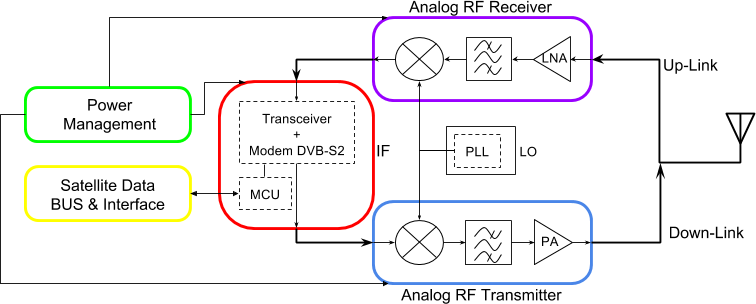
\includegraphics[width=\columnwidth]{figures/SchemaBlocchi}
	\caption{​Block​​ diagram​  of​ ​the​ ​Ka-band​ ​transceiver}
	\label{fig:blo-dia}
\end{figure}
\section{Transceiver architecture}
%%%
The block-diagram of the Ka-band transceiver is given in \cref{fig:blo-dia}.
It is composed by a receiver and a transmitter section sharing a common antenna with polarization diversity.
The Intermediate Frequency (IF) section of both receiver and transmitter provides (accepts) the I/Q samples of the signals to (from) a digital modem, which, in turn, implements in real time all the demodulation, decoding, error correction, and modulation functions of the DVB-2S protocol.
The super-heterodyne receiver exploits a two-stage Low Noise Amplifier (LNA) followed by an image rejection filter: with this configuration the system noise figure is (almost) not affected by the filter losses.
%%%
%%% Waveguide filter no more necessary (remove by the block diagram) ... embedded in the antenna system ...
%%%
%A waveguide filter before the LNA, instead, has the scope to reject the transmitted power. Such a task will be accomplished in conjunction with the antenna interface. To reduce the losses as much as possible, this filter will have an high-pass behaviour, and will be implemented with a waveguide section that is below cut-off at the TX center frequency (\SI{19}{\GHz}) and in propagation at the RX center frequency (\SI{29}{\GHz}).
The transmitter chain is based on an integrated power amplifier with a compression point of 1.5~W.
The amplifier has an integrated power detector, so that power control loop can easily be implemented.
The overall power consumption is around 4.5~W (PAE equal to about 30\%).
%%%
%The transmittersection is characterized by a saturated output power of 1.5~W and features a global power control loop (i.e. from the Ka-band output to the transmitter to its baseband input). To this purpose, a Power Amplifier (PA) with integrated power detector is selected. The overall power dissipation of the PA is around to 4.5~W since the efficiency of the selected Integrated Circuits (ICs) at the compression point is typically around 30\%.
%%%
%%% Verifica la parte sui mixer con Federico Pergolesi ... mi pare che il nuovo sistema utilizzi 2 PLL ...
%%%
Down- and up-conversions are implemented with a couple of twin stand-alone PLLs.
The receiver uses a mixer with integrated frequency doubler for the LO signal ($13 \times 2=26\,\mbox{GHz}$) and has an IF frequency of 3~GHz.
The transmitter, instead, has an IF frequency of 6 GHz and a mixer operating at the fundamental frequency.
Intermediate frequencies can be selected individually up to 6~GHz, thanks to the capabilities of the AD9364 integrated transceiver from Analog Devices \cite{analog}.
This integrated transceiver allows conversion to baseband, AD/DA conversion and data interface.
Its channel bandwidth is of 56~MHz, compatible with the one selected in the link budget.
Should the system require a larger channel bandwidth, the the AD9371 can be adopted.
The digital stream from (to) the AD9364 is then connected with the DVB-S2 modem board.
Redundancy systems, internal interfaces/bus and power managements are included in the design, but not shown in the figure for the sake of clarity.
%%%
% In case of FPGA design, the modem board could also integrate the 6 GHz IF stage (AD9364), in such a way as to have a complete digital back-end. This solution has the advantage to minimize the length of the serial connections between the AD9364 and the FPGA itself, thus maximizing speed and reducing electromagnetic compatibility issues. The external MCU for the transceiver control can also be integrated in the FPGA. The preliminary mechanical concept of the ka-band transceiver is depicted in Figure 2.
%%%
A preliminary set of ICs and devices suitable for the proposed frequencies has already been identified, based on COTS electronic components.
A secondary target of the present research, indeed, is to demonstrate up to what extent commercial electronics can fly successfully in a LEO satellite.
Of particular relevance to this purpose are the families of high-reliability devices nowadays developed for the automotive market.

% The block-diagram of the Ka-band transceiver is given in \cref{fig:blo-dia}.
% It is composed by a receiver and a transmitter section sharing a common antenna with polarization diversity.
% The Intermediate Frequency (IF) section of both receiver and transmitter provides (accepts) the I/Q samples of the signals to (from) a digital modem, which, in turn, implements in real time all the demodulation, decoding, error correction, and modulation functions of the DVB-2S protocol.

% The receiver chain exploits a two-stage Low Noise Amplifier (LNA) in order to achieve a low noise figure.
% This LNA is then followed by the image rejection filter, so that the impact of the filter loss on the noise performance of the receiver is negligible.
% A waveguide filter before the LNA, instead, has the scope to reject the transmitted power.
% % Such a task will be accomplished in conjunction with the antenna interface.
% To reduce the losses as much as possible, this filter will have an high-pass behaviour, and will be implemented with a waveguide section that is below cut-off at the TX center frequency (\SI{19}{\GHz}) and in propagation at the RX center frequency (\SI{29}{\GHz}).
% The transmitter section is characterized by a saturated output power of 1.5~W and features a global power control loop (i.e. from the Ka-band output to the transmitter to its baseband input).
% To this purpose, a Power Amplifier (PA) with integrated power detector is selected.
% The overall power dissipation of the PA is around to 4.5~W since the efficiency of the selected Integrated Circuits (ICs) at the compression point is typically around 30\%.
% Down- and up-conversions are implemented  with a single, stand-alone PLL, operating at about 13 GHz.
% The receiver uses a mixer with integrated frequency doubler for the LO signal (13x2=26~GHz) and has an IF frequency of 3 GHz.
% The transmitter, instead, has an IF frequency of 6 GHz and a mixer operating at the fundamental frequency.
% Intermediate frequencies can be selected individually up to 6~GHz, thanks to the capabilities of the AD9364 integrated transceiver from Analog Devices \cite{analog}.
% This integrated transceiver allows conversion to baseband, AD/DA conversion and data interface.
% Its channel bandwidth is of \SI{56}{\MHz}, compatible with the one selected in the link budget.
% Should the system require a larger channel bandwidth, the the AD9371 can be adopted.
% The digital stream from (to) the AD9364 is then connected with the DVB-S2 modem board.
% Redundancy systems, internal interfaces/bus and power managements are included in the desing, but not shown in the figure for the sake of clarity.
% % In case of FPGA design, the modem board could also integrate the 6 GHz IF stage (AD9364), in such a way as to have a complete digital back-end.
% % This solution has the advantage to minimize the length of the serial connections between the AD9364 and the FPGA itself, thus maximizing speed and reducing electromagnetic compatibility issues.
% % The external MCU for the transceiver control can also be integrated in the FPGA.
% % The preliminary mechanical concept of the ka-band transceiver is depicted in Figure 2.

% A preliminary set of ICs and devices suitable for the proposed frequencies has already been identified, based on commercial, off-the-shelf (COTS) electronic components.
% A secondary target of the present research, indeed, is to demonstrate up to what an extent commercial electronics can fly successfully in a LEO satellite.
% Of particular relevance to this purpose are the families of high-reliability devices nowadays developed for the automotive market.

% % In order to assess the originality of the above architectural design, a brief survey of the Ka-band transceiver state-of-the-art for is now presented.
% % Such a survey is based on three products that reached a commercial maturity and that are specifically designed for small satellites and CubeSats.
% % \begin{itemize}
% % \item Canopus - Aquila Space
% % A Ka-band simplex radio supporting DVB-S2 has been developed by Canopus Systems (later Aquila Space, now Astro Digital), with the support of Sage Millimeter for the IF/RF conversion [4]
% % This system is no longer on the market, as it is part of the platform used by Astro Digital.
% % ​​\item GomSpace
% % The approach followed by GomSpace is to provide two different modules to be mounted on a PC104 compatible motherboard [5,6,7]
% % One of the modules provides a programmable FPGA for the user’s SDR system of preference, while the other includes the IF to RF conversion stage (based on an AD9361 chipset), for RF frequencies up to 6 GHz.
% % \item Tethers Unlimited
% % The SWIFT-KTX is a Ka-band transceiver that can provide high-speed uplink and downlink capability at frequencies of 17-36 GHz with 100 MHz of bandwidth [8]
% % The last information available about the readiness of an engineering unit is Q4 2016, but recent updates are not available.
% % \end{itemize}

% % \begin{figure}[tb]
% % 	\centering
% % 	\missingfigure{figure 2}
% % 	% \includegraphics[width=0.95\textwidth]{}
% % 	\caption{Mechanical concept of the Ka-band transceiver: all the electronics is in a 1.5 U volume.}
% % 	\label{fig:label}
% % \end{figure}

\subsection{RX noise BITE}
\label{sec-RX-noise-bite}
\begin{figure}[tb]
	\centering
	% 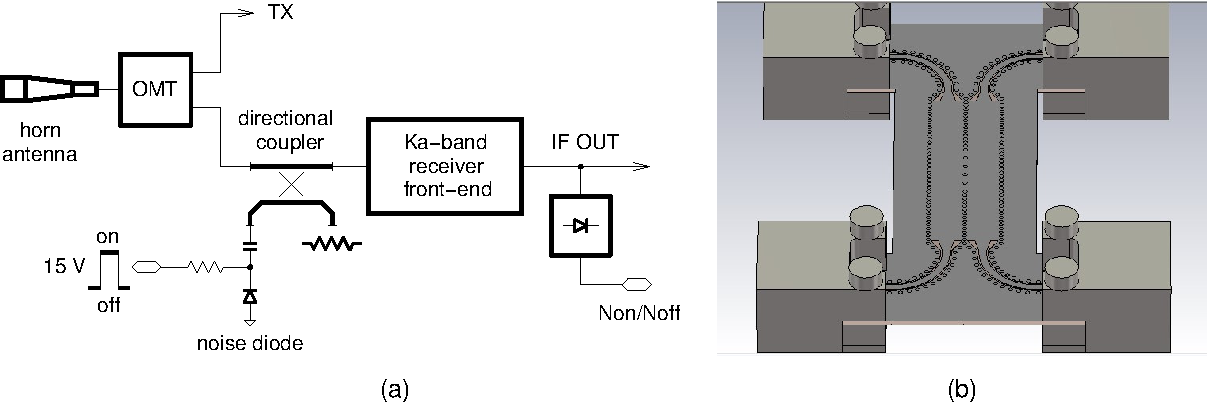
\includegraphics[width=\columnwidth]{figures/fig-noise-bite}
	\subfloat[]{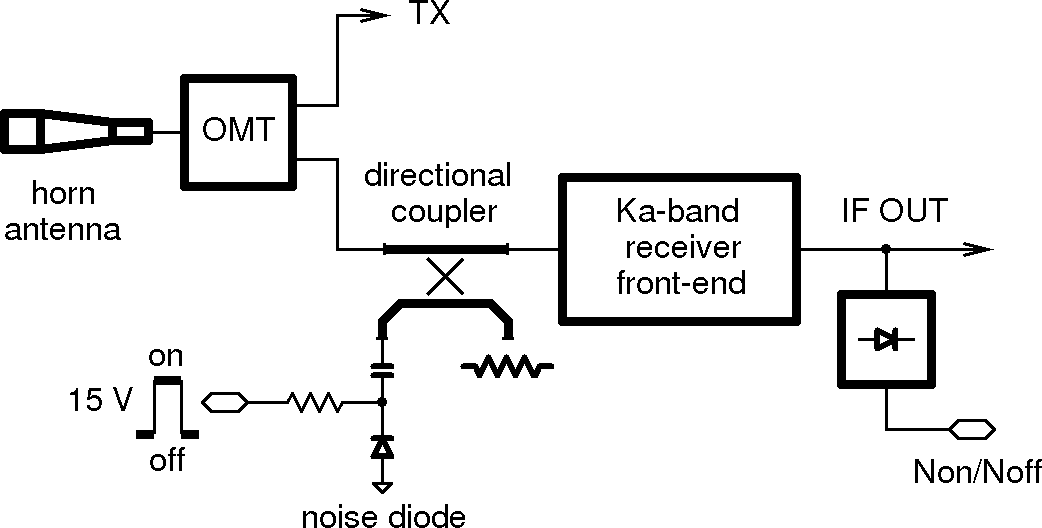
\includegraphics[width=.65\columnwidth,valign=c]{figures/noise-BITE-blk.png}\label{fig:bite-blo-dia}}
	\subfloat[]{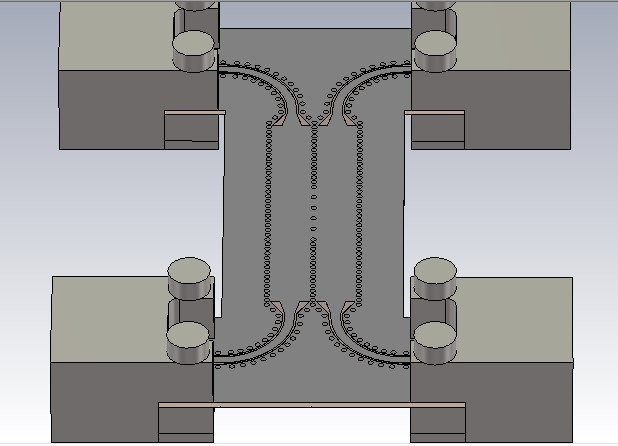
\includegraphics[width=.31\columnwidth,valign=c]{figures/fig-coupler}\label{fig:bite-pro-geo}}
	\caption{Noise BITE block diagram \protect\subref{fig:bite-blo-dia} and geometry of the directional coupler adopted for the noise injection \protect\subref{fig:bite-pro-geo}.
	The directional coupler is designed in SIW technology in order to avoid shields and for superior stability.
	The substrate has a thickness $h=\SI{0.5}{\milli\metre}$ and exploits the Roger 4350B material ($\epsilon_{r}=3.48$, $\tan \delta \simeq 0.004$).
	The active directional coupler length is $l=\SI{15.5}{\mm}$ (uniform waveguide sections included) whereas the waveguide width is $w=\SI{4.3}{\mm}$.
	The via-hole diameter is $d=\SI{0.5}{\mm}$. }
	\label{fig-nbite-geo}
\end{figure}

An original feature of the receiver (RX) sub-system is the possibility to be verified and, possibly, calibrated also during in-orbit operation.
To this purpose a noise BITE is adopted, see \cref{fig-nbite-geo}\subref{fig:bite-blo-dia}.
It is composed by a solid-state avalanche microwave noise source and by a directional coupler connected to the receiver input.
The noise source is controlled by the transceiver CPU.
When the noise source is switched on (high temperature state), a known amount of noise power is injected into the receiver and the corresponding output power, $N_\text{on}$, is measured.
The latter measurement can be implemented in several ways, i.e. by exploiting a zero-bias Schottky diode detector, by using the RSSI output of the IF chip (the AD9364 in our case) or via a suitable processing, once the I/Q signals have been digitally acquired.
Similarly, a receiver output power $N_\text{off}$ is measured when the noise source is switched off (low temperature state).
According to the Y-factor method, \cite{agilent_AN57-1, Alimenti2008}, the overall receiver gain $G_{RX}$ can be evaluated as:
\begin{equation}
   G_{RX} = \frac{N_\text{on} - N_\text{off}}{k_{B}\,C\,\mbox{ENR}\,T_{0}\,B}
   \label{eqn_RX_gain}
\end{equation}
where $k_{B}$ is the Boltzmann constant, $C$ is the coupling factor of the directional coupler, ENR is the Excess Noise Ratio of the avalanche noise source, $T_{0}=290\,\mbox{K}$ is the IEEE standard temperature and $B$ is the bandwidth of the receiver stages before the power detector.
The main advantage of the described procedure is that the gain is determined only exploiting the avalanche noise source: in a laboratory environment the receiver input needs to be simply terminated on a matched load.
During in-orbit operation, instead, the above experiment should be carried out when no signal is received from a ground station.
The \SI{30}{\GHz} receiver antenna (pointed toward the Earth) will behave as a matched load with a physical temperature in the range of \SIrange{150}{300}{\kelvin} (antenna noise temperature).
The noise BITE is designed assuming an injected noise temperature $T_i \simeq C\,\text{ENR}\,T_{0}$ of the same order of magnitude of the antenna noise temperature.
This in order to avoid the receiver saturation during the noise injection phase, and to operate in the linear region of the diode detector (used to measure the output power).
Considering that a 30~GHz avalanche diode has a typical ENR of 20 dB, \cite{noisecom_NC407B,Alimenti2016}, a weak coupling factor $C \simeq -20\,\mbox{dB}$ is needed.
\begin{figure}[tb]
	\centering
	\includegraphics[width=\columnwidth,height=.6\columnwidth]{figures/bite-s-pars}
	% 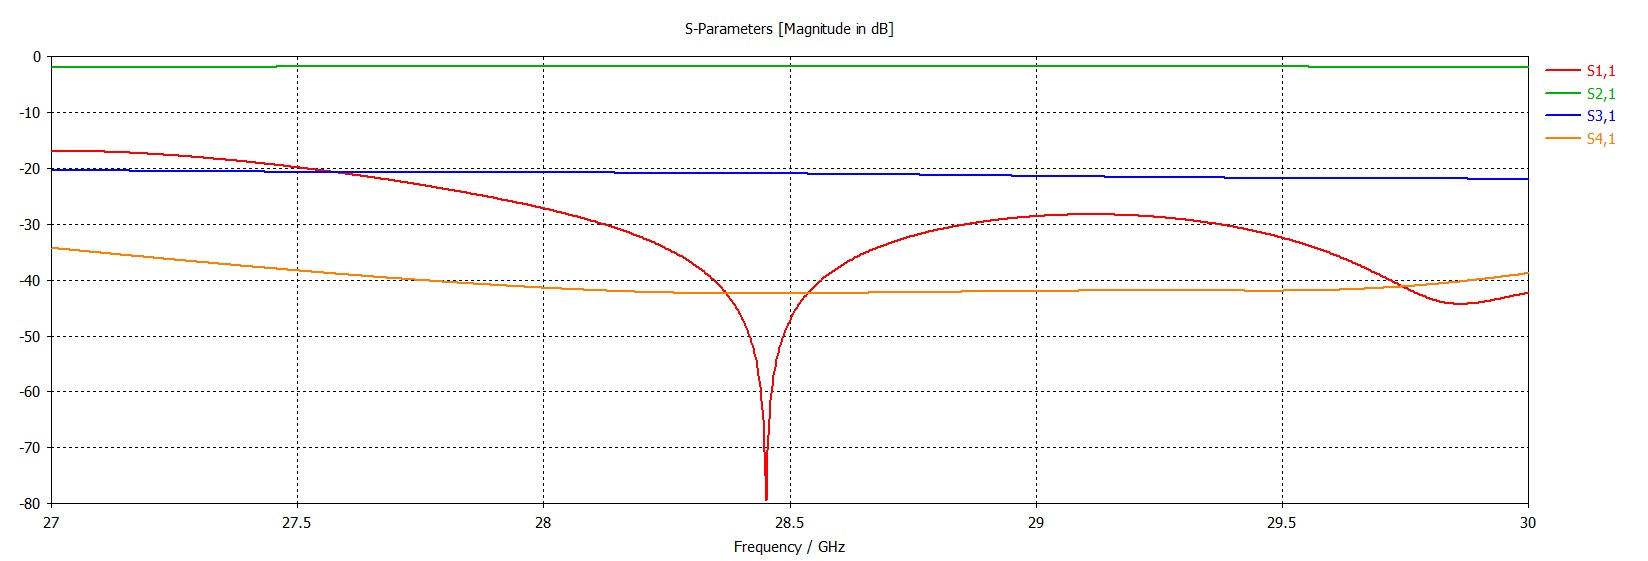
\includegraphics[width=\columnwidth]{figures/fig-coupler-spar}
	\caption{
		Scattering parameters of the SIW directional coupler.
		The full-wave simulations have been carried-out with CST.
		A quite flat coupling $C=-21\,\mbox{dB}$ is obtained at 27.75~GHz (center frequency) with only $1.2\,\mbox{dB}$ roll-off from 27.5 to 30~GHz (receiver full band).
	}
	\label{fig-nbite-res}
\end{figure}
The directional coupler is shown in Fig.~\ref{fig-nbite-geo}(b).
It is implemented in Substrate Integrated Waveguide (SIW) technology~\cite{Doghri2015}; this in order to avoid shields and for superior stability.
A 5-holes side coupling geometry is selected in order to guarantee a wide-band behavior.
The design has been carried-out with CST and the device is optimized paying a particular attention to the insertion losses and to the response flatness.
Four coaxial adapters have been considered in the simulations: this only to be consistent with the experimental characterization.
In the final version the adapters will be removed and the coupler will be completely integrated in the receiver PCB.
The simulation results are shown in Fig.~\ref{fig-nbite-res} for the overall structure (directional coupler with coaxial adapters).
The obtained coupling factor is $C=\SI{-21}{\dB}$ at \SI{27.75}{\GHz} (center frequency) with only \SI{1.2}{\dB} roll-off from \SIrange{27.5}{30}{\GHz} (full receiver band).
This means that the injected noise temperature will be $T_i=\SI{228}{\kelvin}$ for a noise diode with ENR=\SI{20}{\dB}.
The simulated insertion loss is equal to \SI{1.8}{\dB}, i.e. less than \SI{1}{\dB} without coaxial adapter.

\subsection{Co-channel and adjacent channel interference measurements}
A number of measurements has been carried out with the purpose of assessing the BER at the receiver end in presence of a signal interfering on the same channel, or on the adjacent channel.
A range of $C/I$ values, and the presence or absence of noise have been considered.
The test set-up is shown in \cref{fig:interference-dektec-setup}, featuring a Rohde\&{}Schwarz SFC-U modulation generator, to generate the DVB-S2 signal at the center frequency $f_c = \SI{1950}{\MHz}$, an HP8780A signal generator, to generate the interfering signal at the frequency $f_i$, and a DTM-3237 Dektec receiver, compatible with the DVB-S2 protocol.
For each $f_i$, the power level of the interferer was decreased until a correct reception (lock of the receiver) was achieved.
On of the output parameters of the Dektec receiver is $\text{BER}^\dagger$, that is the BER achievable without using the channel coding (consisting of nested LDPC--BCH coding).
The readings of $\text{BER}^\dagger$ were recorded for different values of $C/I$.
Results can be summarized as follows.
The presence of an interferer in the proximity of, or at the center-bandwidth frequency severely affects the reception capability, thus requiring a $C/I \geqslant \SI{6}{\deci\bel}$ to ensure the reception of the transmitted signal (as reported in \cref{fig:ci-meas}), while an offset of at least \SI{10}{\mega\Hz} allows reception at significantly lower $C/I$ levels.
Namely, at $\pm\SI{10}{\MHz}$ from the channel center frequency (\SI{1950}{\MHz}) $C/I \geqslant \SI{-18}{\dB}$ is required, while at $\pm\SI{10}{\MHz}$ this level decreases to \SI{-20}{\dB}.
Nonetheless, a remarkable resistance of the DVB-S2 protocol to interference has been recorded: if the interferer is applied after the signal has been locked, even if the $C/I$ degrades significantly, reception is still possible, and the apparently unsatisfactory $\text{BER}^\dagger$ values (in the order of $10^{-2}$) are well counterweighted by the harsh condition of the interference.
Furthermore, it should be noted that, after the channel decoding, the communication is error-free, whichever the value considered in \cref{fig:ci-meas}, provided that the transmitted signal is locked by the receiver.
In addition, if $f_i$ is outside the channel bandwidth of the transmitted signal, the reception is error-free for any $C/I$ attainable with the proposed setup.
\begin{figure}[tb]
	\centering
	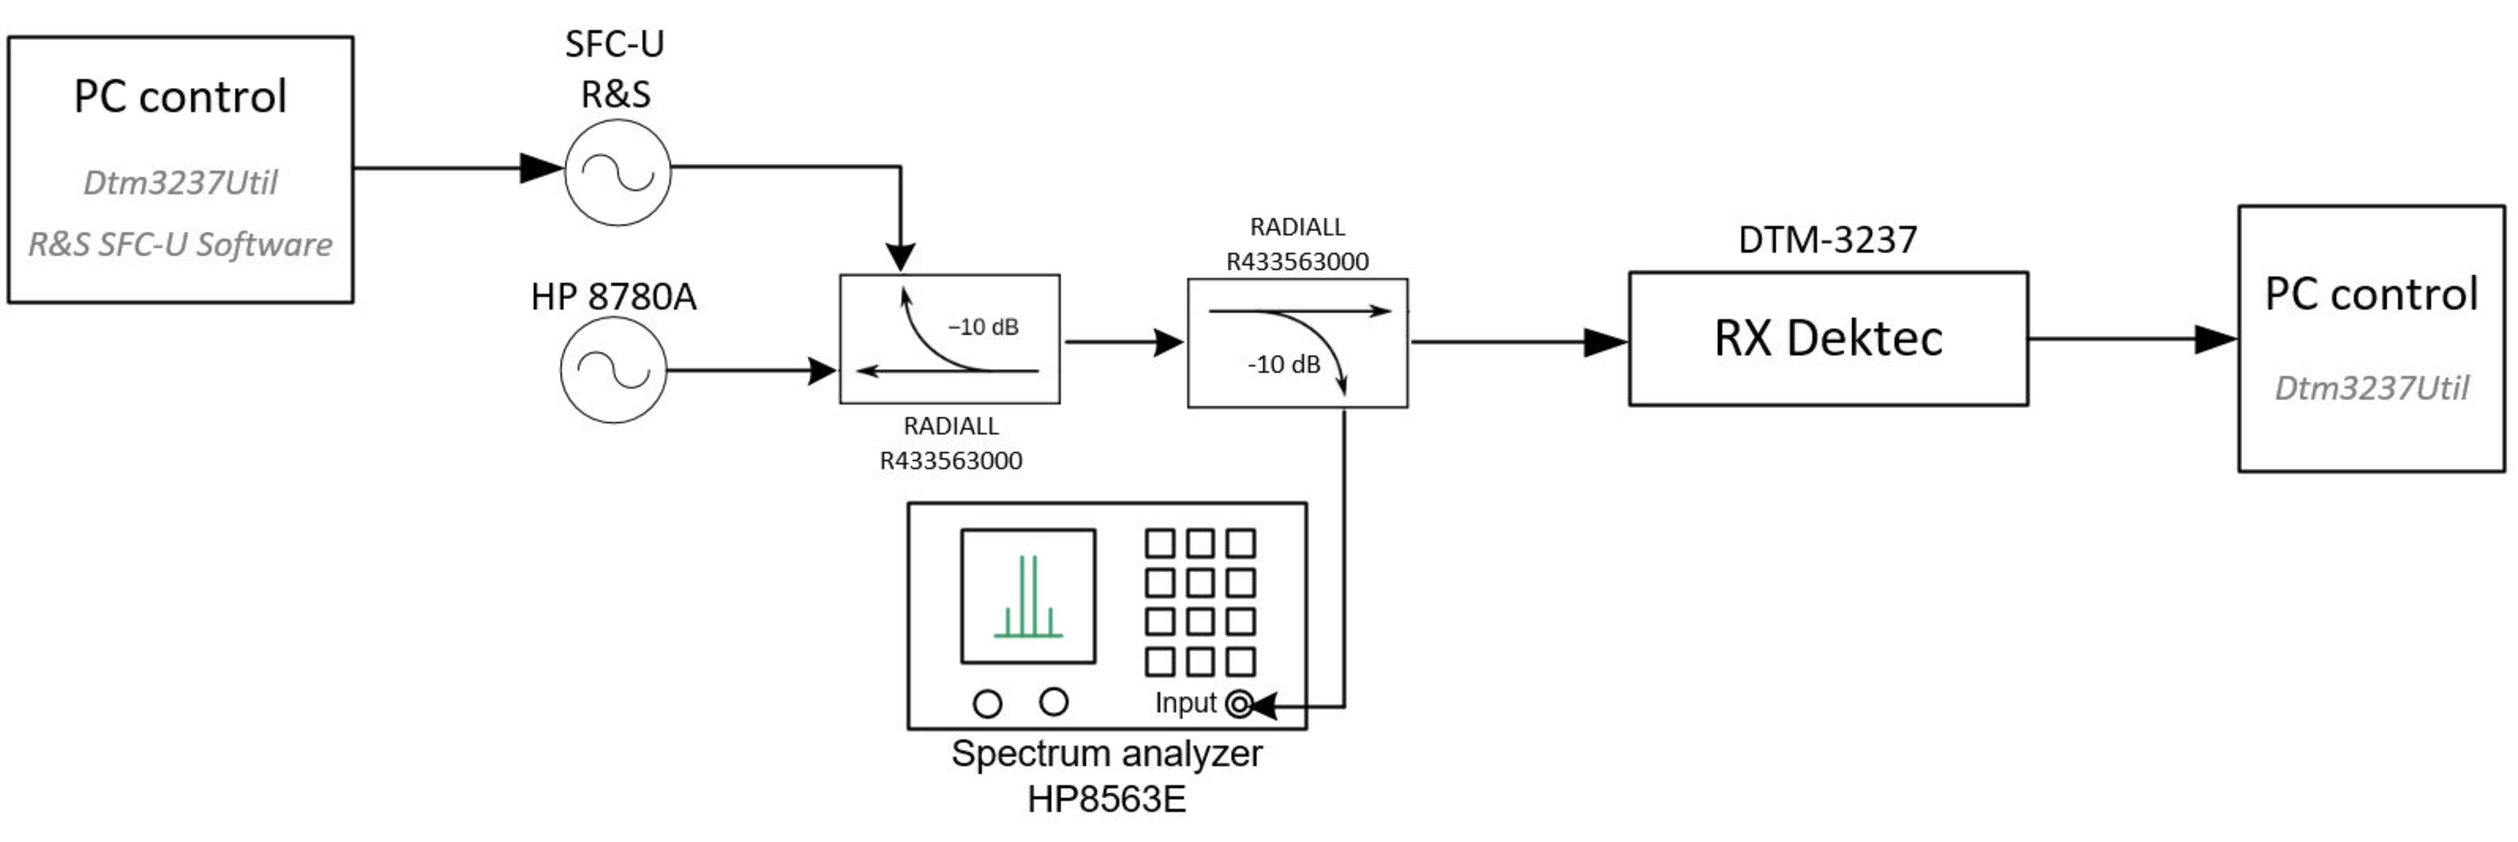
\includegraphics[width=\columnwidth]{figures/interference-dektec-setup}
	\caption{Setup for the interference measurements.}
	\label{fig:interference-dektec-setup}
	\vspace{\baselineskip}
	\includegraphics[width=\columnwidth,height=.7\columnwidth]{figures/ber-vs-ci}
	\caption{$C/I$ measurements. For $f_i = \SI{1950}{\mega\Hz}$ and $C/I = [0,6]~\si{\deci\bel}$, $\text{BER}^\dagger = 0$ (error-free), and the values are not plotted.}
	\label{fig:ci-meas}
\end{figure}
% \begin{table}[tb]
% 	\centering
% 	\footnotesize
% 	\caption{List of the $C/I$ levels required for reception (${C/I}_l$) at different interferer frequencies $f_i$. }
% 	\label{tab:lock-levels}
% 	\begin{tabular}{cc}
% 	\toprule
% 	$f_i$ [\si{\mega\Hz}] & ${C/I}_l$ [\si{\deci\bel}] \\
% 	\toprule
% 	$1927$ & $< -20$ \\
% 	\midrule
% 	$1940$ & $-18$ \\
% 	\midrule
% 	$1950$ & $6$ \\
% 	\midrule
% 	$1960$ & $-18$ \\
% 	\midrule
% 	$1973$ & $< -20$ \\
% 	\bottomrule
% 	\end{tabular}
% \end{table}

\section{Antenna concept}
\label{sec:ant-des}
The antenna is a wide-band corrugated horn that operates in circular polarization: left-hand for the RX (27.5-30~GHz) and right-hand for the TX (17.8-20.2~GHz) channels respectively
% (see Fig.~\ref{fig-antenna})
.
These two channels are separated via a dual-band polarizer and an orthomode transducer (OMT).
The horn shape is designed and optimized accounting for: i) gain of 20~dBi minimum; ii) low side-lobes; iii) low cross-polarization (1~dB main beam); iv) volume and mass reduction.
The horn profile is synthesized in order to minimize the spurious mode conversion and the depth of the grooves has been defined in order to optimize both the input matching and the pattern symmetry~\cite{Teniente2002}.
A square corrugated waveguide with thick irises is the key design features of the dual-band polarizer~\cite{Liu2008}.
The polarizer is then connected to the OMTs by means of a diamond transition, which rotates the irises of 45~deg. with respect to the ports of the OMT.
In the present design the OMT act also as TX/RX diplexer.
It uses a dual junction configuration in order to optimize the input matching and the port-to-port isolation~\cite{DArcangelo2009}.
The isolation is further increased exploiting the cutoff of the circular waveguide in the TX band, while the isolation between RX and TX bands is obtained by means of a corrugated filter placed into the receiving branch.
The proposed antenna, besides consisting of waveguide elements, is proving to be a promising approach, as it requires a single horn only.
Other techniques can also be considered in terms of compactness and manufacturability, as proposed in \cite{Buttazzoni2017}.

% The antenna system depicted in figure 2 shows two branches, one for the uplink (Tx, at 27.5-30 GHz) and the other for the downlink (Rx, at 17.8-20.2 GHz) in circular polarization, left hand and right hand respectively.
% The satellite link is achieved by a single wide band corrugated horn connected to a dual band polarizer and two orthomode transducers (OMTs).

% A shaped corrugated horn has been designed in order to obtain the following performances in the overall frequency band (17.8 – 30 GHz):
% \begin{itemize}
% \item high directivity (minimum Gain > 20dBi from the link budget)
% \item low side lobes
% \item good input matching
% \item low cross polarization within 1dB main beam (pointing error)
% \item manufacturing feasibility
% \item overall length compatible with the satellite module dimensions
% \end{itemize}
% The horn has been designed with CAE/FEM tools; the profile of the horn has been synthesized in order to minimize the spurious mode conversion and the depth of the grooves has been defined in order to optimize both the input matching and the pattern symmetry \cite{Teniente2002}.

% The polarizer is a device aimed to convert a linear polarization to a circular one.
% In particular, two linear orthogonal polarizations become two circular polarizations (left hand and right hand).
% In the present case the two circular polarization of the Tx and Rx band are converted into linear polarizations to be picked up by the OMT/Diplexer connected to the branches of the transceiver.
% A square corrugated waveguide with thick irises are the key design features of such polarizer, which have been optimized to obtain a good axial ratio within the Tx and Rx sub bands.
% The goal is to have an axial ratio performance in agreement with cross polarization requirements envisaged in the link budget \cite{Liu2008}.
% The polarizer is then connected to the OMTs by means of a diamond transition, which rotates the irises of 45 degrees with respect to the ports of the OMT.

% The OMT separates two orthogonal linear polarizations that, in the present case, are relevant to the different Tx and Rx frequency bands.
% Therefore, the OMT behaves as a frequency diplexer.
% A dual junction configuration has been chosen to optimize the input matching and the port-to-port isolation in the frequency bands.
% The design has been carried with CAE/FEM tools \cite{DArcangelo2009}.
% The isolation between Tx and Rx bands is obtained thanks to the cutoff performances of the circular waveguide in the Tx band, while the isolation between Rx and Tx bands is obtained by means of a corrugated filter placed into the receiving branch.
% A properly designed septum is positioned to define reflection section for the Rx band.
% The output ports match with the Tx and Rx branches of the transceiver and the overall dimensions of the OMT must satisfy the mechanical constraints of the satellite module.
\begin{figure}[tb]
	\centering
	\includegraphics[width=\columnwidth,height=.7\columnwidth]{figures/horn-rad-pat}
	% 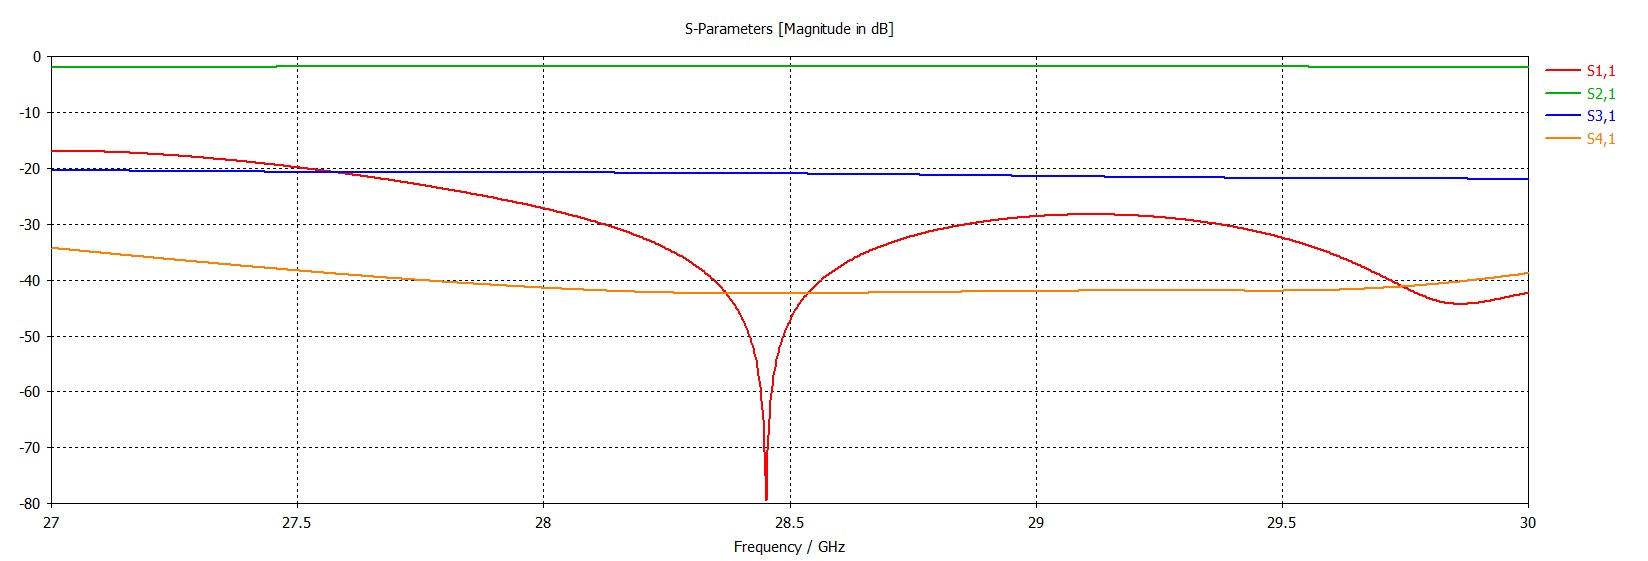
\includegraphics[width=\columnwidth]{figures/fig-coupler-spar}
	\caption{Horn antenna radiation patterns at the center frequencies.}
	\label{fig:rad-pat}
\end{figure}

\section{Conclusions}
\label{sec:con}
This paper shows that a Ka-band transceiver
 % (uplink 29~GHz, downlink 19~GHz)
for CubeSats can be implemented using COTS components.
It is capable of 100~Mbps data rate with a volume of 1.5~U and consumption of 20~W.
The transmitted power is 1.5~W and a 20~dBi, dual-band antenna (corrugated horn, polarizer and OMT) is adopted.
A noise BITE allows to check the receiver gain during operation.
Exploiting a communication interface like this, new horizons could be opened for low-cost space missions.

\section*{Acknowledgment}
The authors acknowledge the European Space Agency for its technical support in this work within the contract no. 4000117224/16/UK/AD.

\bibliographystyle{IEEEtran}
\bibliography{IEEEabrv,references}

\end{document}